% UTF-8 encoding
\documentclass{beamer} %
% Beamer 设置
%\usetheme[secheader]{Boadilla} % 使用的 Beamer 主题: Boadilla
%\usecolortheme{beaver} % 使用的 Beamer 颜色:beaver

\usetheme{Warsaw}
\usefonttheme[onlymath]{serif}
% 字体设置
%\usefonttheme{professionalfonts} % professional 字体

% 其他 Package
\usepackage{times}
\usepackage{amsmath}
\usepackage{verbatim}
\usepackage{anyfontsize}
\usepackage{subcaption} % 子图片
\usepackage{graphicx} % 图片
\usepackage[export]{adjustbox}
\setbeamertemplate{caption}[numbered]
\newcounter{saveenumi}
\resetcounteronoverlays{saveenumi}
\usepackage[multidot]{grffile} % 允许文件名带多个点
\usepackage{tabularx} % 表格
\usepackage{tikz}
\usepackage{ctex}
\usepackage{multicol}
\usepackage{mathtools} % 提供 \mathcolorbox
\usepackage{xcolor}    % 提供颜色支持
\usepackage{braket} % Dirac 符号
\AtBeginSection[]
{
	\begin{frame}{Index}
		\transfade%淡入淡出效果
		\tableofcontents[sectionstyle=show/shaded,subsectionstyle=show/shaded/hide]
		\addtocounter{framenumber}{-1}  %目录页不计算页码
	\end{frame}
}
%%%%%%%%%%%%%%%%%%%

\title{暗物质存在的证据与可能的解释 } % 标题
\author{林照翔  } % 作者
\date{\today} % 如果 Date 参数为空,自动显示当前日期

\begin{document}
\songti %宋体
\setbeamerfont{headline}{size=\Tiny}
\everymath{\displaystyle}

    % 标题页
\begin{frame}
    \titlepage % 根据上面信息生成标题
\end{frame}

\begin{frame}
    \frametitle{\textbf{Index}}
    \begin{multicols}{2}
    \tableofcontents
    \end{multicols}
\end{frame}

\section{引言}

\begin{frame}{引言}
在现代宇宙学和粒子物理学的发展中,暗物质(Dark Matter)问题被视为最根本而深刻的未解之谜之一。尽管它无法通过电磁相互作用被直接观测,我们却可以通过大量天文现象间接推断出其存在:从星系旋转曲线的异常,到引力透镜效应的质量分布不符,再到宇宙微波背景辐射和大尺度结构的形成。暗物质在宇宙演化中扮演着不可或缺的角色。

暗物质的概念最早可以追溯到1930年代,当时Fritz Zwicky发现,可见星系的质量不足以提供星系团内所需的引力约束。随后,1970年代Vera Rubin对螺旋星系的系统观测进一步确立了“质量不守恒”的现象,并引发对宇宙中“不可见物质”的广泛研究。此后,暗物质逐渐被纳入ΛCDM(Λ Cold Dark Matter)模型,成为标准宇宙学框架中不可或缺的一环。
\end{frame}

\begin{frame}
然而,迄今为止,暗物质的本质仍不明确。尽管从引力效应可以推断出其存在,我们却尚未直接探测到暗物质粒子。其成分、相互作用类型乃至是否真为“物质”本身,仍是理论物理和实验物理的重大前沿课题。对此,物理学界提出了多种理论模型,如WIMP(弱相互作用大质量粒子)、轴子、超对称模型和额外维等,并开展了大量直接与间接探测实验。

本文旨在对暗物质研究进行简要综述,围绕观测证据与理论模型两条主线展开。第二章将介绍三类主要的暗物质观测证据,包括星系旋转曲线、引力透镜效应以及宇宙微波背景辐射;第三章将介绍当前主流的暗物质候选者,讨论它们的物理动机、特点与局限;第四章则简要介绍正在进行中的实验努力及其最新进展;第五章将讨论当前研究所面临的挑战及未来可能的发展方向。

通过综述现有观测结果与理论探索,本文希望为理解暗物质的研究路径提供清晰的结构与概览,并凸显该问题在现代物理中的核心地位与挑战性。
\end{frame}

\section{暗物质存在的观测证据}

\subsection{星系旋转曲线(Galaxy Rotation Curves)}

\begin{frame}
星系旋转曲线是指星系中恒星和气体的圆周速度随其距离星系中心变化的曲线。它反映了星系内部质量分布对恒星和气体运动的影响。

星系旋转曲线有两种测量方法。光谱学方法:通过测量星系中恒星和气体的光谱线,可以确定它们的多普勒位移,从而计算出它们的径向速度。结合星系的几何结构,可以推导出恒星和气体的圆周速度;射电天文学方法:利用射电望远镜观测星系中的中性氢(HI)气体发射的21厘米线,可以确定气体的运动速度。这种方法特别适用于观测星系的外边缘区域,因为这些区域的恒星密度较低,光学观测较为困难。
\end{frame}

\begin{frame}
1914年,Wolf和Slipher发现仙女座星系(M31)的光谱线在星系主轴方向上倾斜,在短轴方向上则为直线,从而得出仙女座星系在旋转的结论。

1939年,Horace Babcock在他的博士论文中,测量了仙女座星系的旋转曲线,发现其在大半径处的圆周速度非常高,暗示星系外侧存在大量质量。

自1970年代起,Vera Rubin 和 Kent Ford 等人对多个螺旋星系的旋转曲线进行观测,发现实际数据与经典预言严重不符:在远离星系中心的区域,恒星的轨道速度并未下降,而是趋于平坦。这意味着在星系外围区域仍存在大量未被观测到的质量,其引力足以维持恒星的高速旋转。
\end{frame}

\begin{frame}
\begin{figure}[!htbp]
    \centering    
    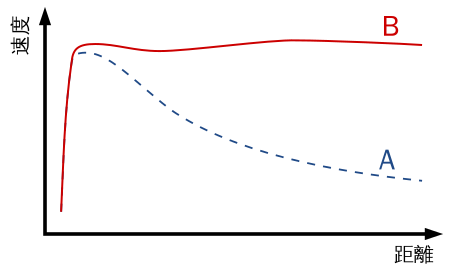
\includegraphics[height=3cm]{Img/2-1.png}
    \caption{星系旋转曲线:预测的(A)和观测的(B)。 }
    \label{2-1}
\end{figure}

根据牛顿引力定律,如果星系的质量主要集中在可见的恒星和气体中,那么随着到星系中心距离的增加,恒星和气体的圆周运动速度应该逐渐下降。然而,观测到的星系旋转曲线在大半径处保持平坦,这表明在星系的外围存在大量未被观测到的质量,这些质量无法用可见的恒星和气体来解释,从而为暗物质的存在提供了有力证据。
\end{frame}

\subsection{引力透镜效应(Gravitational Lensing)}

\begin{frame}
根据广义相对论,质量分布可以导致时空弯曲,进而使背景天体发出的光线发生偏折,这一现象称为引力透镜效应。在天文学中,引力透镜被用作测量系统总质量的重要手段,尤其是在星系团尺度。

\begin{figure}[!htbp]
    \centering    
    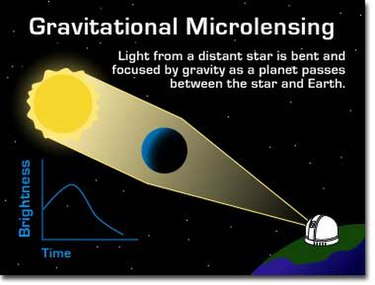
\includegraphics[height=4cm]{Img/2-2.jpg}
    \caption{引力透镜效应 }
    \label{2-2}
\end{figure}
\end{frame}

\begin{frame}
通过对多个星系团的引力透镜效应进行分析,可以发现引力作用远远超过可见物质所能提供的水平。例如,在著名的子弹星系团(Bullet Cluster)中,两个星系团发生高速碰撞:X射线观测显示热气体集中在中心,而引力透镜揭示的质量分布却偏移至两个星系团的外围部分。换言之,引力“重心”不在可见质量重心所在的位置。这一现象被广泛认为是“可见物质无法解释全部引力作用”的直接证据。引入“不可见但有质量”的暗物质成分能够自然地解释质量分布与光偏折之间的关系。此外,弱引力透镜在大范围宇宙尺度上也支持类似结论:通过引力透镜效应观测得到的总质量普遍高于可见质量之和。
\end{frame}

\subsection{宇宙微波背景(Cosmic Microwave Background)}

\begin{frame}
1965年,Arno Penzias和Robert Wilson在贝尔实验室进行射电天文学研究时,意外地发现了一种来自宇宙各个方向的均匀背景辐射。这种辐射的温度约为2.7 K,频率分布符合黑体辐射的谱线。这一发现被确认为宇宙微波背景辐射(Cosmic Microwave Background, CMB),为大爆炸理论提供了直接的观测证据。

宇宙微波背景辐射是大爆炸残留下的热辐射,携带着早期宇宙密度扰动的信息。通过对CMB各个多极谱峰的位置与高度进行精密测量(如 WMAP、Planck 计划),研究者可以推断宇宙的基本成分比例。
\end{frame}

\begin{frame}
\begin{figure}[!htbp]
    \centering    
    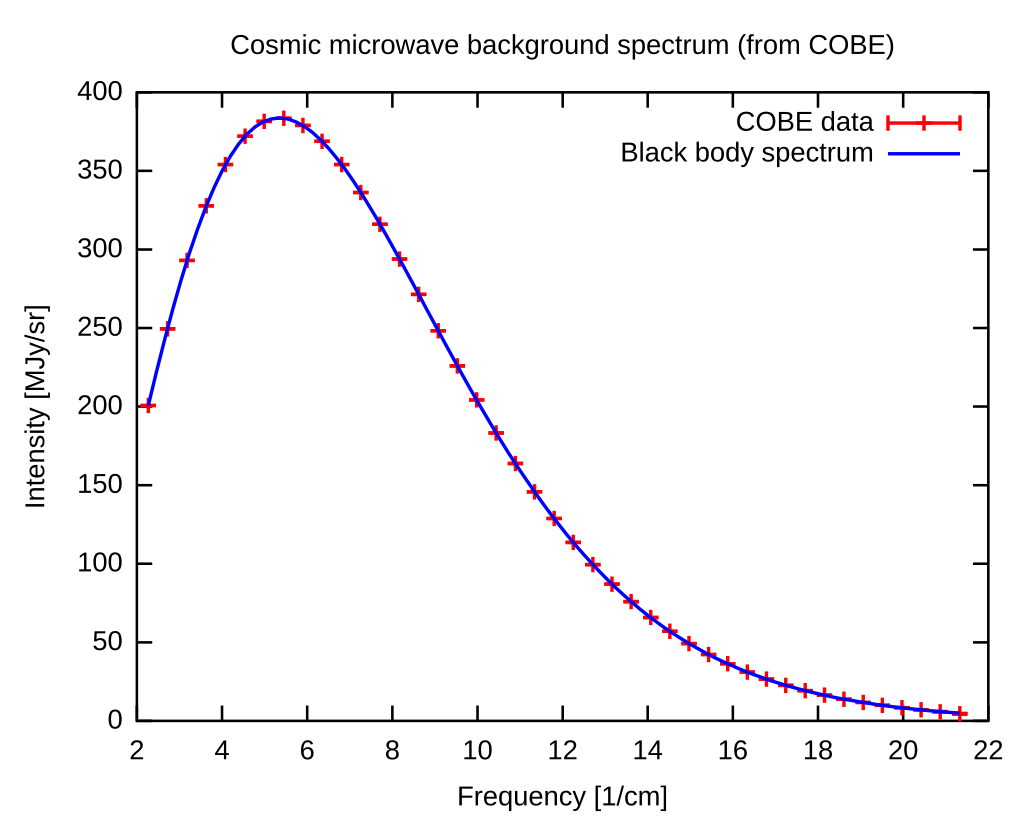
\includegraphics[height=2.8cm]{Img/2-3.png}
    \caption{由FIRAS仪器对COBE观测的宇宙微波背景辐射光谱 }
    \label{2-3}
\end{figure}

暗物质的存在会改变CMB功率谱的形状。通过分析CMB功率谱,可以推断出宇宙的总物质密度、暗物质密度和可见物质密度等宇宙学参数。这些测量结果与星系旋转曲线、引力透镜效应等其他观测结果一致,为暗物质的存在提供了有力证据。

CMB的温度分布存在微小的涨落,这些涨落反映了宇宙早期的密度不均匀性。通过分析CMB的温度涨落,可以推测宇宙的总物质密度、暗物质密度和可见物质密度。CMB的观测结果表明,暗物质约占总物质密度的85\%,而可见物质仅占15\%左右。
\end{frame}

\section{暗物质的候选者}

\subsection{WIMP:弱相互作用大质量粒子(Weakly Interacting Massive Particles)}

\begin{frame}
根据目前流行的宇宙学模型,早期宇宙处于高温状态,各种粒子通过快速交换能量处于热平衡态粒子数密度满足玻尔兹曼分布,宇宙的温度随着其膨胀而逐渐下降,直到今天的温度为3K 左右。在温度下降的过程中,与热力学平衡体系相互作用较弱的稳定粒子会在某个时期脱离热平衡,其粒子数密度不再随温度而快速下降,成为剩余丰度。这些剩余粒子最终形成今天宇宙中存在的各类基本元素。这一热退耦机制很好地解释了宇宙中的轻元素比如氦的丰度。暗物质作为一种弱相互作用的粒子,其丰度也有可能是来源于热力学退耦。研究表明,如果暗物质的相互作用强度和质量在电弱能标附近,可以自然解释宇宙中的暗物质丰度。这一类候选者通常被称为弱相互作用大质量粒子(WIMP)。
\end{frame}

\begin{frame}
在WIMP类暗物质丰度的计算中,由于存在各种数量级上差别巨大的物理量如 CMB温度、哈勃常数、普朗克常数等的偶然相消,导致了最后要求的暗物质质量在电弱质量标度附近,而很多新物理理论模型中预期的暗物质质量也正好在电弱质量标度附近。这种巧合被称为 WIMP “奇迹”(WIMP miracle)。

假设稳定的暗物质粒子为 $X$,它和标准模型粒子 $Y$ 通过 $X\bar{X} \leftrightarrow Y\bar{Y}$ 进行反应。这个过程可以由玻尔兹曼方程来描述

\begin{align}
\frac{\mathrm{d}n_X }{\mathrm{d}t } + 2 H n_X 
=-\braket{\sigma_{X\bar{X}}\left|v \right|} \left(n_X^2 - n_{X,\mathrm{eq}}^2 \right),
\end{align}

其中,$n_X$ 是暗物质粒子的数密度;$n_{X,\mathrm{eq}}$ 是处于热平衡的粒子数密度;$H\equiv \dot{R}/R=\left(8\pi G \rho/3 \right)^{1/2}$ 是宇宙的膨胀速度;$\braket{\sigma_{X\bar{X}}\left|v \right|}$ 是暗物质湮灭截面的热平均值。当宇宙早期的温度远大于 $m_X$ 时,$X\bar{X}$ 的产生和湮灭过程达到动态平衡,所以暗物质和标准模型粒子一样大量存在。
\end{frame}

\begin{frame}
随着宇宙的膨胀,宇宙温度逐渐降低。当温度降至 $m_X$ 以下时,标准模型粒子 $Y$ 不能有效碰撞产生暗物质粒子 $X$,这是因为假设 $Y$ 按能量分布是玻尔兹曼分布,当温度低于 $m_X$ 时,能量大于 $m_X$ 的粒子是指数下降的。而暗物质粒子的湮灭过程仍在继续,所以 $X$ 粒子数密度在迅速降低。一般来讲,$X$ 是非相对论粒子,此时 $X$ 粒子的平衡密度为

\begin{align}
n_{X,\mathrm{eq}}
=g_X \left(\frac{m_X T}{2\pi }  \right)^{3/2} \mathrm{e}^{-m_X/T},
\end{align}

其中 $g_X$ 是 $X$ 拥有的内部自由度的数目。当宇宙降温至某个温度 $T_f$ 以下时,暗物质湮灭过程发生的速度小于宇宙膨胀速度,即 $n \Braket{\sigma_{X\bar{X}}\left|v \right|} \leqslant H .$ 可认为暗物质再膨胀的几率很小,其数密度基本只受宇宙膨胀的影响,即达到热退耦(thermal freeze-out),相应的温度 $T_f$ 称为退耦温度。
\end{frame}

\begin{frame}
通过求解玻尔兹曼方程,可以近似得到今天宇宙中暗物质残留密度

\begin{align}
\Omega_X h^2 \sim g_*^{-1/2} x_f \frac{1.17\times 10^{-10} }{a+3b/x_f }, 
\end{align}

其中 $a,b$ 来自暗物质湮灭截面的非相对论展开 $\Braket{\sigma_{\bar{X}X}\left|v \right|}=a+b\Braket{v^2}+\mathcal{O}\left(v^4 \right)$;与宇宙温度相关的变量 $x_f$ 的定义是 $x_f\equiv m_X/T$;$g_*$ 是一个外部自由度(在标准模型中,在 $T\sim 1~\mathrm{TeV}$ 时,$g^*\sim 120$;在 $T\sim 1~\mathrm{GeV}$ 时,$g^*\sim 65$)。

如果要求上面假设的过程能够解释今天观测到的暗物质残留密度,即 $\Omega_X h^2 \sim 0.11$,则可以对暗物质的湮灭截面有个大概的估计(只考虑湮灭截面里与速度无关的部分,并假设 $g_*\sim 100,x_f\sim 20$)
\end{frame}

\begin{frame}
\begin{align}
\Braket{\sigma_{X\bar{X}}\left|v \right|}
\sim g_*^{-1/2} x_f \frac{1.17 \times 10^{-10} ~\mathrm{GeV}^{-2} }{\Omega_x h^2 } \sim 10^{-9}~\mathrm{GeV}^{-2}, 
\end{align}

而通常一种质量为 $m_X$,相互作用耦合常数为 $\alpha$ 的粒子的湮灭截面可以近似写为(假设 $\alpha\sim 0,01,m_X\sim 300~\mathrm{GeV}$)

\begin{align}
\sigma_{X\bar{X}} \sim \frac{\alpha^2 }{m_X^2 } \sim 10^{-9}~\mathrm{GeV}^{-2},
\end{align}

这就是说,如果暗物质质量在 GeV-TeV 范围,且电弱相互作用的量级 $\alpha\sim 0.01$,那么它的数密度就符合目前实验观测。这就是所谓的WIMP“奇迹”。
\end{frame}

\subsection{轴子(Axion)}

\begin{frame}
自上世纪七十年代以来,物理学家在夸克模型假设下在用规范场理论来描写强相互作用方面作了巨大努力,建立了称为量子色动力学的理论。量子色动力学可以很好地解释一些现象,但也存在一些困难。其中一个困难就是破坏了宇称守恒和时间反演不变性,这与实验事实矛盾。为了摆脱这一困境,理论物理学家提出了两种可能的路径:一种是假设夸克的质量为零,另一种是假设有一种轻的、长寿命的、不带电的玻色子存在,这种玻色子就是轴子(Axion)。我们知道,夸克是是自然界所有物质的最基本的组成单元,其质量不可能为零。因此轴子的假设可能更为合理。
\end{frame}

\begin{frame}
根据理论上的推断,轴子可能的自旋值和宇称为 $0^-,1^+,2^-,3^+,\cdots$,它的质量为

\begin{align}
m_a
\approx 25 N \left(x+\frac{1 }{x }  \right)~\mathrm{keV},
\end{align}

其中 $N$ 是夸克二重态的数目,其至少为 $2$;$x$ 是理论中引入的一个自由参变量。当自由参变量 $x=1$ 时,$x+1/x$ 有最小值 $2$,因此轴子的质量 $m_a$ 至少是 $100~\mathrm{keV} .$

轴子的寿命与它的质量有密切的关系。当轴子的质量小于两倍电子质量时,它只能通过放射两个 $\gamma$ 光子的方式衰变

\begin{align}
a \to \gamma + \gamma,
\end{align}
\end{frame}

\begin{frame}
它的寿命可以表示为

\begin{align}
\tau_{a\to 2\gamma}
\approx 0.4 Z^{-1} \left(\frac{100~\mathrm{keV} }{m_a }  \right)^5~\mathrm{s},
\end{align}

其中 $Z\equiv m_u/m_d \approx 0.56$,$m_u$ 是上夸克的质量,$m_d$ 是下夸克的质量。若 $m_a\approx 100~\mathrm{keV}$,则它的寿命大约是 $0.7~\mathrm{s} .$

若轴子的质量大于两边电子质量,那么除了放射两个 $\gamma$ 光子的衰变方式之外,衰变方式

\begin{align}
a \to e^+ + e^-,
\end{align}

也是允许的。这样轴子的寿命就会短很多。理论上给出轴子通过放射 $e^+ e^-$ 偶衰变方式的寿命为
\end{frame}

\begin{frame}
\begin{align}
\tau_{a\to e^+ e^-}
=\frac{8 \pi x^2 f_\phi^2}{m_e^2\left(m_a^2-4m_e^2 \right)^{1/2} } ,
\end{align}

其中 $f_\phi\equiv \left(\sqrt{2} G_F \right)^{-1/2}$,$G_F$ 是费米耦合常数;$m_e$ 是电子质量。若取 $x\approx 1$,那么当轴子质量 $m_a$ 为几 MeV 时,轴子通过放射 $e^+ e^-$ 偶衰变方式的寿命 $\tau_{a\to e^+ e^-}$ 大约是 $10^{-8} - 10^{-9}~\mathrm{s} .$
\end{frame}

\begin{frame}
轴子能够作为暗物质的原因主要包括以下几点:

1. 解决强 CP 问题的机制:轴子源自佩奇-奎恩(PQ)机制,作为一种伪-诺恩-戈尔登(pseudo-Nambu-Goldstone)玻色子出现,能够自然解释强相互作用中的 CP 破缺问题(强 CP 问题)。其存在由粒子物理理论预测,具有很强的理论基础。

2. 早期宇宙中的产生机制:在宇宙早期,通过“真空重整机制”、弦和壁的衰变等过程,轴子以冷暗物质的形式在宇宙中生成。这些冷轴子没有与其他粒子充分热平衡,因此表现出无温度的、冷暗物质的特性,符合暗物质的要求。

3. 极长的相干长度和低能量尺度:轴子具有极小的质量(在微电子伏特范围),对应非常低的动能和长的相干长度,使得它们在银河系尺度上表现为高度相干的场,这符合暗物质的分布特征。
\end{frame}

\begin{frame}
4. 与引力和其他暗物质特性兼容:轴子作为无电荷、无磁矩、互动弱的粒子,不与普通物质发生强烈相互作用,符合暗物质不与电磁辐射直接相互作用的特性。

5. 密度和宇宙演化的一致性:轴子在宇宙中的粮食密度和结构形成中扮演角色,能够支持银河系中的暗物质候选粒子的角色,并且与宇宙学观察(如宇宙微波背景辐射、星系旋转曲线等)观察结果相一致。

因此,轴子凭借其产生机制、物理性质和宇宙分布的兼容性,被认为是极佳的暗物质候选粒子。
\end{frame}

\subsection{超对称模型 (Supersymmetry Model)}

\begin{frame}
目前,基本粒子之间的相互作用是由标准模型来描述的。这样的理论基于量子力学基本原理、狭义相对论、杨-米尔斯局域规范作用和最小作用量原理。

量子力学基本原理提供了量子化概念,狭义相对论和杨-米尔斯局域规范作用分别对应全局时空对称性和局域内禀对称性,最小作用量原理指导如何从满足以上对称性的拉式量得到运动方程。

上面提到的对称性分为全局的和局域的。全局变换对称性是指对场做常数变化(变化量不是时间空间的函数)情况下,作用量不变。局域变换对称性是指对场做局域变化(变化量可以是是时间空间的函数)情况下,作用量不变。
\end{frame}

\begin{frame}
标准模型具有的对称性为 $P\otimes G$,其中 $P$ 表示庞加莱群,即四维时空的洛伦兹变换加上时空平移变换。在标准模型中,认为庞加莱对称性是全局的。如果要将其局域化,则涉及到广义相对论和引力。由于粒子需要满足庞加莱不变性,于是庞加莱群决定了可以存在的粒子的种类,即每种粒子可以按群的基本表示归类。

后面的 $G$ 表示内禀对称性,在标准模型中,$G=\mathrm{SU(3)_c \otimes SU(2)_L \otimes U(1)_Y }$,并且是局域对称性。局域对称性 $G$ 描述了标准模型里的强、弱以及电磁相互作用。在标准模型中,根据以上对称性写出拉式量,并根据最小作用量原理就可以得到各种粒子的运动方程。
\end{frame}

\begin{frame}
超对称模型是近年来最为流行的一种超出标准模型的新物理模型。超对称模型与标准模型的唯一不同在于将前面的庞加莱群 $P$ 换为更大的时空对称性 $S$,超对称代数。超对称代数包含了庞加莱群,并且加入了玻色子和费米子的反对易变换操作。同样的,在这里 $S$ 是作为全局对称性处理的,如果考虑局域化的超对称代数 $S$,则是超引力(Supergravity)的研究范围.由于 $S$ 是一个更大的时空对称性,超对称包含的粒子数比标准模型要多,每一个粒子都有其超对称伴子(玻色子的超对称伴子是一个费米子,反之亦然)。
\end{frame}

\begin{frame}
超对称的引入能够解决在 Higgs 粒子质量的圈图修正计算中遇到的等级问题,并且可以使各种规范作用常数在高能标处达到统一。

在早些时候,为了解决超对称模型里质子衰变的问题引入了 $R$ 宇称,其定义为 $R\equiv (-1)^{3B+L+2S}$,其中 $B,L,S$ 分别为重子数、轻子数和自旋。所有的标准模型粒子和超对称粒子分别具有偶宇称 $R=+1$ 和奇宇称 $R=-1$,因此所有的超对称粒子必须成对产生或消灭,这样最轻的超对称粒子(lightest supersymmetry particle, LSP)就是稳定的,可以作为暗物质的候选者。

超对称粒子的质量谱是由超对称破缺的细节来决定的。但是,在超对称粒子列表里能够成为暗物质候选者的粒子并不多。
\end{frame}

\begin{frame}
在最小超对称模型里,具有电中性、色中性的粒子是四种 neutralino(中性规范玻色子以及 Higgs 粒子的超对称伴子),三种sneutrino(中微子的超对称伴子)以及 gravitino(引力子graviton的超对称伴子)。

在不加入右手中微子的情况下,sneutrino不能做为暗物质候选者,因为它大大超过了目前直接探测的限制,已经被目前直接探测实验排除。

Gravitino是合适的暗物质候选者它与其他粒子的相互作用极其微弱,不被目前已有的实验限制,但是因此对它的探测也相当困难。

Neutralino是超对称中研究最广泛的粒子。在超对称模型中,四种标准模型的超对称伴子(bino、wino和两个中性higgsino)混合后组成的四个质量本征态被称为neutralino,其中最轻的neutralino即是暗物质候选者。
\end{frame}

\subsection{额外维 (Extra Dimensions) }

\begin{frame}
额外维模型假设真实的时空并非通常的3+1维,而是具有更高的维度。这些额外的维度很小,因此不为我们所知。

最早的 ADD模型里就包括由 n 个小于毫米量级的平坦的额外维度。在 ADD模型里引力在全空间里传播,而标准模型粒子则限制在四维膜(四维空间在高维空间中的切片)上。这样的设置下,在长距离的情况下,引力行为和以前相同。但是,在距离和额外维的大小差不多时,引力的行为就会出现偏离,因此得出的普朗克能标比以前低。通过适当的参数选取,可以使普朗克能标降到 TeV 量级,这样就解决了前面提到的 Higgs粒子质量的圈图修正计算中遇到的等级问题。
\end{frame}

\begin{frame}
在稍后提出的 Randall-Sundrum 模型里,依旧引入的是极小尺度的额外维,不过它们具有很大的空间曲率和 ADD 模型相同,RS模型中的引力在全空间里传播,而标准模型粒子则限制在四维膜上。在 RS 模型中,所有基本的物理参数都可以是四维普朗克能标量级大小,但是由于空间曲率引起的卷曲因子,这些物理参数在标准模型四维膜上都被压低到 TeV 量级。这同样解决了Higgs粒子质量的等级问题。

普朗克能标降到 TeV 量级的另一个重要意义是解释了为什么我们观测到的引力作用强度比其他三种力强、弱、电磁力要小很多。由于牛顿引力系数与普朗克质量平方成反比,当普朗克质量为 TeV 量级时,引力与弱电相互作用强度相当。这样使得在额外维模型里面,自然界四种力强、弱、电磁、引力的相互作用强度是差不多的。那么为什么我们观测到的引力比其他三种力要小呢? 因为时空存在更多维度,而引力存在于所有维度.我们作为四维时空的观测者只看到一部分的引力,所以强度变小了。用形象的话来说,引力“漏”到其他维度里面去了。
\end{frame}

\begin{frame}
由于以上两个模型只有引力在全空间里传播,因此引入的新粒子主要是一些激发态的引力子 graviton.

普遍的额外维模型(universal extra dimensions,UED)则假设平坦的额外维,但是所有的标准模型粒子都在空间的所有维度中传播。在 UED 模型中,额外维的大小由于实验限制以及理论原因通常取为 $R^{-1} \sim \mathrm{TeV}^{-1} .$ 标准模型粒子在额外维中传播可能带有动量,于是在四维膜上表现为新的重粒子,即 Kaluza-Klein(KK) 激发态。由于额外维上的周期边界条件,在额外维的动量是量子化的.所以,KK 激发态在树图层次上的质量为

\begin{align}
m_{X^{(n)}}^2
=\frac{n^2 }{R^2 } + m_{X^{(0)}}^2,
\end{align}

其中,$X^{(n)} $ 是标准模型粒子的第 $n$ 个 KK 激发态;$R^{-1}\sim \mathrm{TeV}^{-1} $ 是额外维的大小;$X^{(0)}$ 是标准模型粒子,也是 KK 态的基态。在这个模型中,粒子的 KK激发态一般在 TeV,这个能标与目前 PAMELA和 ATIC 实验感兴趣的暗物质质量范围很接近。
\end{frame}

\begin{frame}
最轻的 KK粒子的稳定性通常由 KK 宇称守恒保证。通常一个额外维假设被紧致为一个圆环 $S$(即 $r=0$ 的点和 $r=R$ 的点是同一个点),两个额外维会紧致为两个一维圆环的直积,即圆环面。在这种紧致下,额外维的动量守恒使得 KK 数($n$) 是守恒的。但是,在实际模型中为了构建手征费米子,额外维取为 $S/Z_2$($x\leftrightarrow -x$ 的对径捏合)或者 $T^2/Z_2$ 迹形(orbifold)。这个设置破坏了 KK 数($n$)的守恒,但是仍然存在 KK宇称守恒,即 $n$ 的奇偶性守恒仍保留下来。在 KK 宇称下为奇的质量最轻的粒子(lightest KK particle),比如光子的第一 KK 激发态,是稳定的,可以作为暗物质的候选者。
\end{frame}

\section{暗物质探测实验现状}

\begin{frame}
暗物质的探测手段可以分为直接探测实验和间接探测实验。直接探测实验,即通过探测暗物质粒子与实验靶核子的散射来确定暗物质的存在;间接探测实验,即探测暗物质湮灭或衰变产生的各种粒子,从而确定暗物质的存在。

直接探测的基本思想是:若暗物质粒子(如 WIMP)穿过地球时与原子核发生弹性散射,可在地下探测器中留下微弱信号。由于背景噪声(如宇宙射线、天然放射性)极高,因此这些实验通常建在深地下实验室中,以屏蔽干扰。

间接探测的目标是寻找暗物质湮灭或衰变产生的产物,如高能 $\gamma$ 射线、反质子、正电子或中微子。这类信号通常来源于暗物质密度较高区域,如银河中心或星系团。
\end{frame}

\subsection{DAMA 实验组}

\begin{frame}
银河系被认为由一个均匀分布的暗物质晕(halo)包围,暗物质粒子在其中随机热运动。太阳系绕银河中心公转的速度约为 220 km/s,形成了一个“暗物质风”。地球则绕太阳公转,速度约为 30 km/s。

地球在 每年6月的运动方向与太阳运动方向一致,与“暗物质风”相对速度最大。在 每年12月,两者方向相反,与“暗物质风”相对速度最小。暗物质粒子与探测器中原子核的弹性散射率和能量沉积随速度变化,从而导致探测率呈现一年周期的调制。DAMA 使用 高纯度碘化钠闪烁晶体(NaI(Tl)) 作为探测器,监测中低能核反冲事件的计数率。数据处理过程中排除日常背景变化和伽马射线等非WIMP事件的影响,关注随时间变化的微弱周期信号。
\end{frame}

\begin{frame}
\begin{figure}[!htbp]
    \centering    
    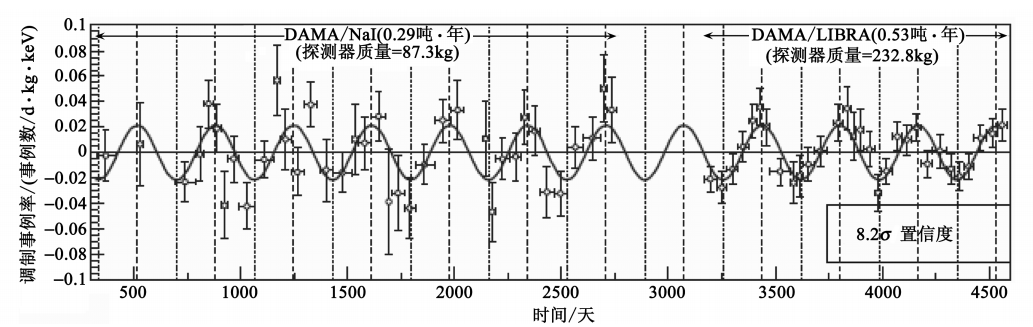
\includegraphics[height=3cm]{Img/4-1.png}
    \caption{DAMA 实验观测到的年调制信号.这有可能是来自于暗物质碰撞的信号 }
    \label{4-1}
\end{figure}

然而,除了 DAMA 实验组外,其他实验组均未看到暗物质碰撞的正面信号,暗物质的信号至今还未被其他实验所证实。
\end{frame}

\subsection{PAMELA 实验组}

\begin{frame}
2008 年,欧洲的 PAMELA 卫星实验公布了宇宙线中反物质的探测结果,显示地球附近太空中的正电子能谱在能量约高于10GeV 的区域内明显上升,与传统的宇宙线理论预言的下降能谱不符合,同时该实验组在能量约低于100GeV 的能区内未探测到超出背景的反质子。

\begin{figure}[!htbp]
    \centering    
    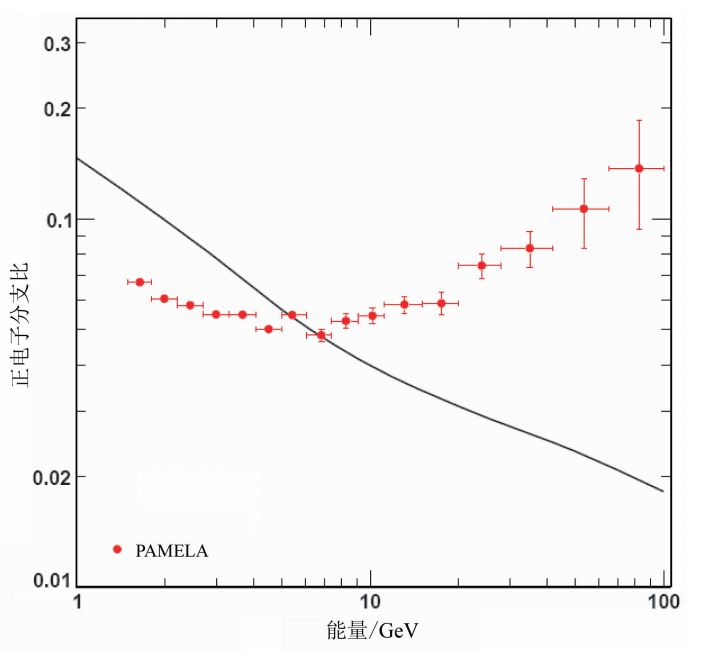
\includegraphics[height=2cm]{Img/4-2.png}
    \caption{PAMELA 卫星实验观测结果。实线对应理论背景预期结果,红点为实验观测数据。 }
    \label{4-2}
\end{figure}

很多研究者试图用暗物质来解释正电子的超出,但是为了避免反质子的超出,必须接受一个结果即暗物质的湮灭主要产生轻子对,而不是夸克对。这对传统的暗物质模型提出了挑战。
\end{frame}

\subsection{ATIC 实验组}

\begin{frame}
ATIC 使用的是高空气球平台,飞行高度约为 35–40 km,能在大气层之上长时间运行(特别是在南极可以利用极夜形成的平流层气流循环,飞行时间达几周)。其主要目标是测量宇宙线中电子(包括正电子)通量与能谱。

\begin{figure}[!htbp]
    \centering    
    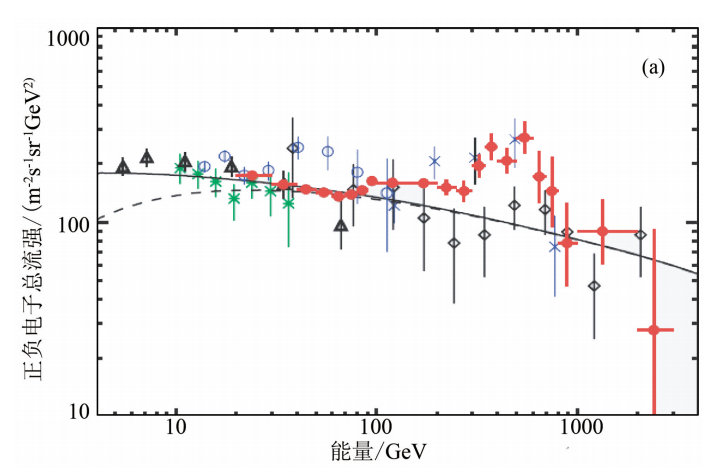
\includegraphics[height=2cm]{Img/4-3.png}
    \caption{ATIC 实验组2008年公布的正负电子流量的数据。红色数据点为 ATIC 在2008年公布的数据,其余数据点为之前实验测量数据;实线和虚线为不同理论模型给出的正负电子流量的背景预测值。 }
    \label{4-3}
\end{figure}

ATIC 实验组观测到正负电子流量之和在 300 GeV 到 800 GeV 有一个明显超出,并且能谱有明显鼓包结构。这种异常可能来源于暗物质。
\end{frame}

\section{总结}

\begin{frame}
暗物质作为现代宇宙学与粒子物理交汇处最重要的问题之一,已成为连接宏观宇宙结构与微观基本粒子的关键线索。从1930年代Zwicky首次提出“隐藏质量”假说,到今日多波段、多手段观测支持下ΛCDM模型的建立,暗物质研究走过了近一个世纪的探索历程。当前,星系旋转曲线、引力透镜效应与宇宙微波背景辐射等多重观测证据已牢固确立了暗物质存在的事实。然而,它的基本属性、粒子本质以及相互作用机制仍未被揭示。

理论上,WIMP、轴子等多种候选粒子模型在标准模型之外提供了丰富的可能性,但在LHC、XENON、LUX-ZEPLIN、AMS-02等一系列前沿实验的努力下,尚无确凿的探测信号被确认。与此同时,ATIC、PAMELA、DAMPE 和 AMS 等间接探测实验对正电子、反质子等能谱结构的观测则引发了关于天体源与暗物质湮灭机制的激烈讨论,也暴露出理论建模的不确定性与观测解释的多义性。
\end{frame}

\begin{frame}
展望未来,暗物质研究正迈向更高灵敏度与多探针协同发展的阶段。实验方面,下一代液氙探测器(如DARWIN)、空间谱仪(如HERD)以及地下超低本底实验(如PANDAX-III)将显著提升对WIMP和轻暗物质的探测能力。理论方面,更加重视宇宙学-粒子物理-引力三者融合的跨尺度建模,也将成为理解暗物质本质的关键突破口。此外,若未来某一实验或观测方向取得决定性结果,其影响将不仅局限于暗物质本身,更可能推动标准模型和广义相对论的根本性修正。

因此,尽管当前我们尚未“看见”暗物质,但它正以前所未有的方式引领基础物理学走向更深层的理解,揭示关于宇宙、物质和引力的基本奥秘。
\end{frame}

\end{document}